\section{Proposed Framework Overview}
\label{sec:framework_overview}

This chapter details the systematic methodology employed in this research to develop and evaluate an adaptive detection framework for fileless and polymorphic malware. The core of the proposed approach integrates techniques from memory forensics, computer vision, and machine learning to overcome the limitations of traditional detection methods when faced with these evasive threats. The framework operates by analyzing the runtime state of processes captured within volatile memory dumps, transforming this data into a visual format amenable to image-based feature extraction, and applying machine learning for classification.

The overall workflow, visually summarized in Figure \ref{fig:methodology_overview}, consists of four primary phases:

\begin{enumerate}
    \item \textbf{Phase 1: Memory Analysis (Data Acquisition and Preparation):} This initial phase involves setting up a controlled environment, executing potentially malicious Portable Executable (PE) files, and capturing full memory dumps at runtime. These binary memory dumps are then systematically converted into standardized RGB image representations.
    \item \textbf{Phase 2: Feature Extraction:} From the generated RGB images, distinctive visual features are extracted using a combination of computer vision descriptors. Specifically, global features using GIST \citep{oliva2001modeling} and local features using HOG \citep{dalal2005histograms} are computed and fused into a single, high-dimensional feature vector representing the visual characteristics of the memory dump.
    \item \textbf{Phase 3: Multi-Class Classification:} The fused feature vectors are used to train and evaluate various machine learning classifiers (e.g., Linear SVM, SMO, XGBoost, Random Forest, J48). The goal of this phase is to accurately classify samples into their respective malware families or as benign, based on the learned visual patterns.
    \item \textbf{Phase 4: Unknown Malware Detection Enhancement:} To specifically address the challenge of zero-day threats, the UMAP \citep{mcinnes2018umap} manifold learning technique is applied. UMAP reduces the dimensionality of the feature space while aiming to preserve significant data structures. Classifiers are then trained on this reduced space using known malware data and evaluated on their ability to detect unknown malware families introduced only during the testing phase, typically in a binary (malware vs. benign) classification setup.
\end{enumerate}

This multi-phase approach allows for a comprehensive analysis, leveraging the exposure of malware behavior in memory and the pattern recognition capabilities of computer vision and machine learning. The subsequent sections provide detailed descriptions of the system architecture, environmental setup, and the specific implementation steps undertaken within each phase of this framework.

% --- Placeholder for the Mermaid diagram figure environment ---
\begin{figure}[h!]
  \centering
  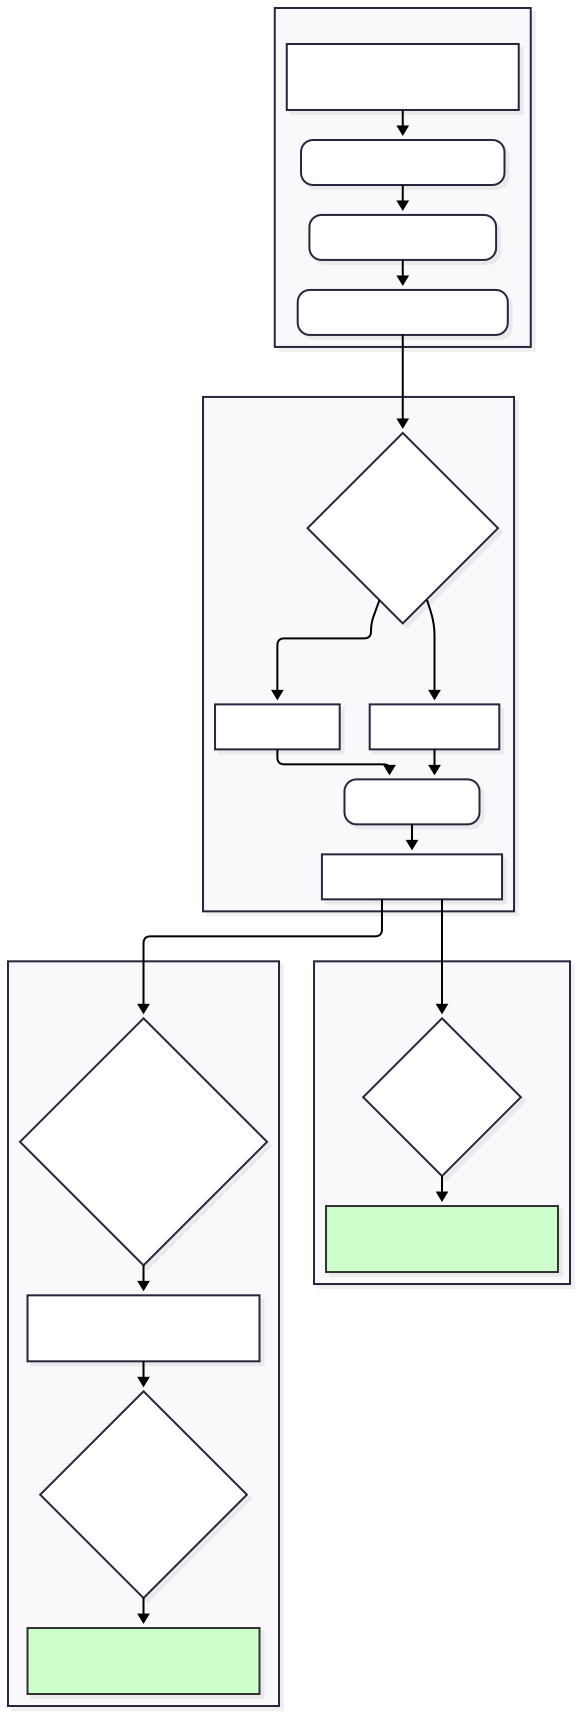
\includegraphics[width=0.8\textwidth]{../Assets/3-1.svg}
  \caption{High-level overview of the proposed malware detection framework.}
  \label{fig:methodology_overview}
\end{figure}
% --- End Placeholder ---

\section{System Architecture and Setup}
\label{sec:system_setup}

To effectively analyze the behavior of fileless and polymorphic malware and collect memory artifacts, a controlled and robust experimental environment was established. This section details the hardware specifications, virtualization platform, operating systems, and key software tools utilized throughout the research.

\subsection{Hardware Environment}
\label{subsec:hardware}

The experiments were conducted on a physical host machine equipped with sufficient resources to support virtualization and computationally intensive tasks such as image processing and machine learning model training. The key hardware components of the host system included:
\begin{itemize}
    \item \textbf{Processor (CPU):} An Intel Core i7 processor was used, providing adequate computational power for running multiple virtual machines and processing large memory dumps[cite: 79].
    \item \textbf{Memory (RAM):} The host system was equipped with 16GB of RAM[cite: 79]. This capacity was crucial for allocating sufficient memory to guest virtual machines to ensure reliable memory dump acquisition, particularly aiming to minimize fragmentation effects potentially caused by techniques like Address Space Layout Randomization (ASLR)[cite: 67]. A minimum of 16GB was allocated to the virtual machines themselves during the memory dump collection phase[cite: 67].
    \item \textbf{Graphics Processing Unit (GPU):} An NVIDIA T1000 GPU was available on the system[cite: 79]. While the core feature extraction (GIST/HOG) and traditional ML model training (SVM, RF, etc.) are often CPU-bound, the presence of a capable GPU can be beneficial for accelerating certain machine learning tasks or potential future work involving deep learning models.
    \item \textbf{Storage:} Sufficient storage space was allocated for storing the operating system images, virtual machine snapshots, collected memory dumps (which could range from 1GB to several GBs each [cite: 60]), generated images, extracted features, and experimental results.
\end{itemize}

\subsection{Software and Virtualization Environment}
\label{subsec:software}

A virtualized sandbox environment was essential for safely executing and analyzing potentially malicious software samples without risking harm to the host system or network. One can refer to \ref{fig:system_setup} for a overview.
\begin{itemize}
    \item \textbf{Hypervisor:} VMWare ESXI was employed as the virtualization platform[cite: 67]. ESXI is a bare-metal hypervisor providing efficient resource management and isolation capabilities suitable for creating secure analysis environments.
    \item \textbf{Guest Operating Systems:} Virtual machines running Microsoft Windows 10 and Windows 11 were deployed within the ESXI environment[cite: 67]. Using both operating systems allows for analysis across different recent Windows versions where fileless and polymorphic malware are prevalent.
    \item \textbf{Memory Acquisition Tool:} Microsoft's ProcDump utility (version 9.0) was the primary tool used for capturing memory dumps[cite: 60]. It was specifically configured using the `-ma` parameter to capture a full process dump, including the process's entire virtual address space[cite: 60].
    \item \textbf{Analysis Environment:} Data processing, image conversion, feature extraction, and machine learning experiments were primarily conducted using Python. Key libraries likely included scientific computing libraries (like NumPy, SciPy), image processing libraries (like Pillow, OpenCV), machine learning libraries (like Scikit-learn, XGBoost), and potentially the UMAP library implementation. A modified version of the "bin2png" Python script was specifically used for the memory dump to image conversion process[cite: 62].
    \item \textbf{Endpoint Monitoring:} An Endpoint Detection and Response (EDR) system was monitored during malware execution within the sandbox to confirm successful execution before initiating the memory dump capture[cite: 60]. This helped ensure that the captured memory state reflected the active malware behavior.
\end{itemize}

This setup provided a controlled, isolated, and well-resourced environment for collecting high-quality memory dumps from malware execution and subsequently performing the image conversion, feature extraction, and classification tasks central to this research methodology.

% --- Optional Mermaid Diagram Placeholder ---
% Suggestion: A simple block diagram showing Host -> ESXI -> (Win10 VM + ProcDump, Win11 VM + ProcDump) -> Memory Dumps -> Python Analysis Environment (Host)
\begin{figure}[h!]
  \centering
  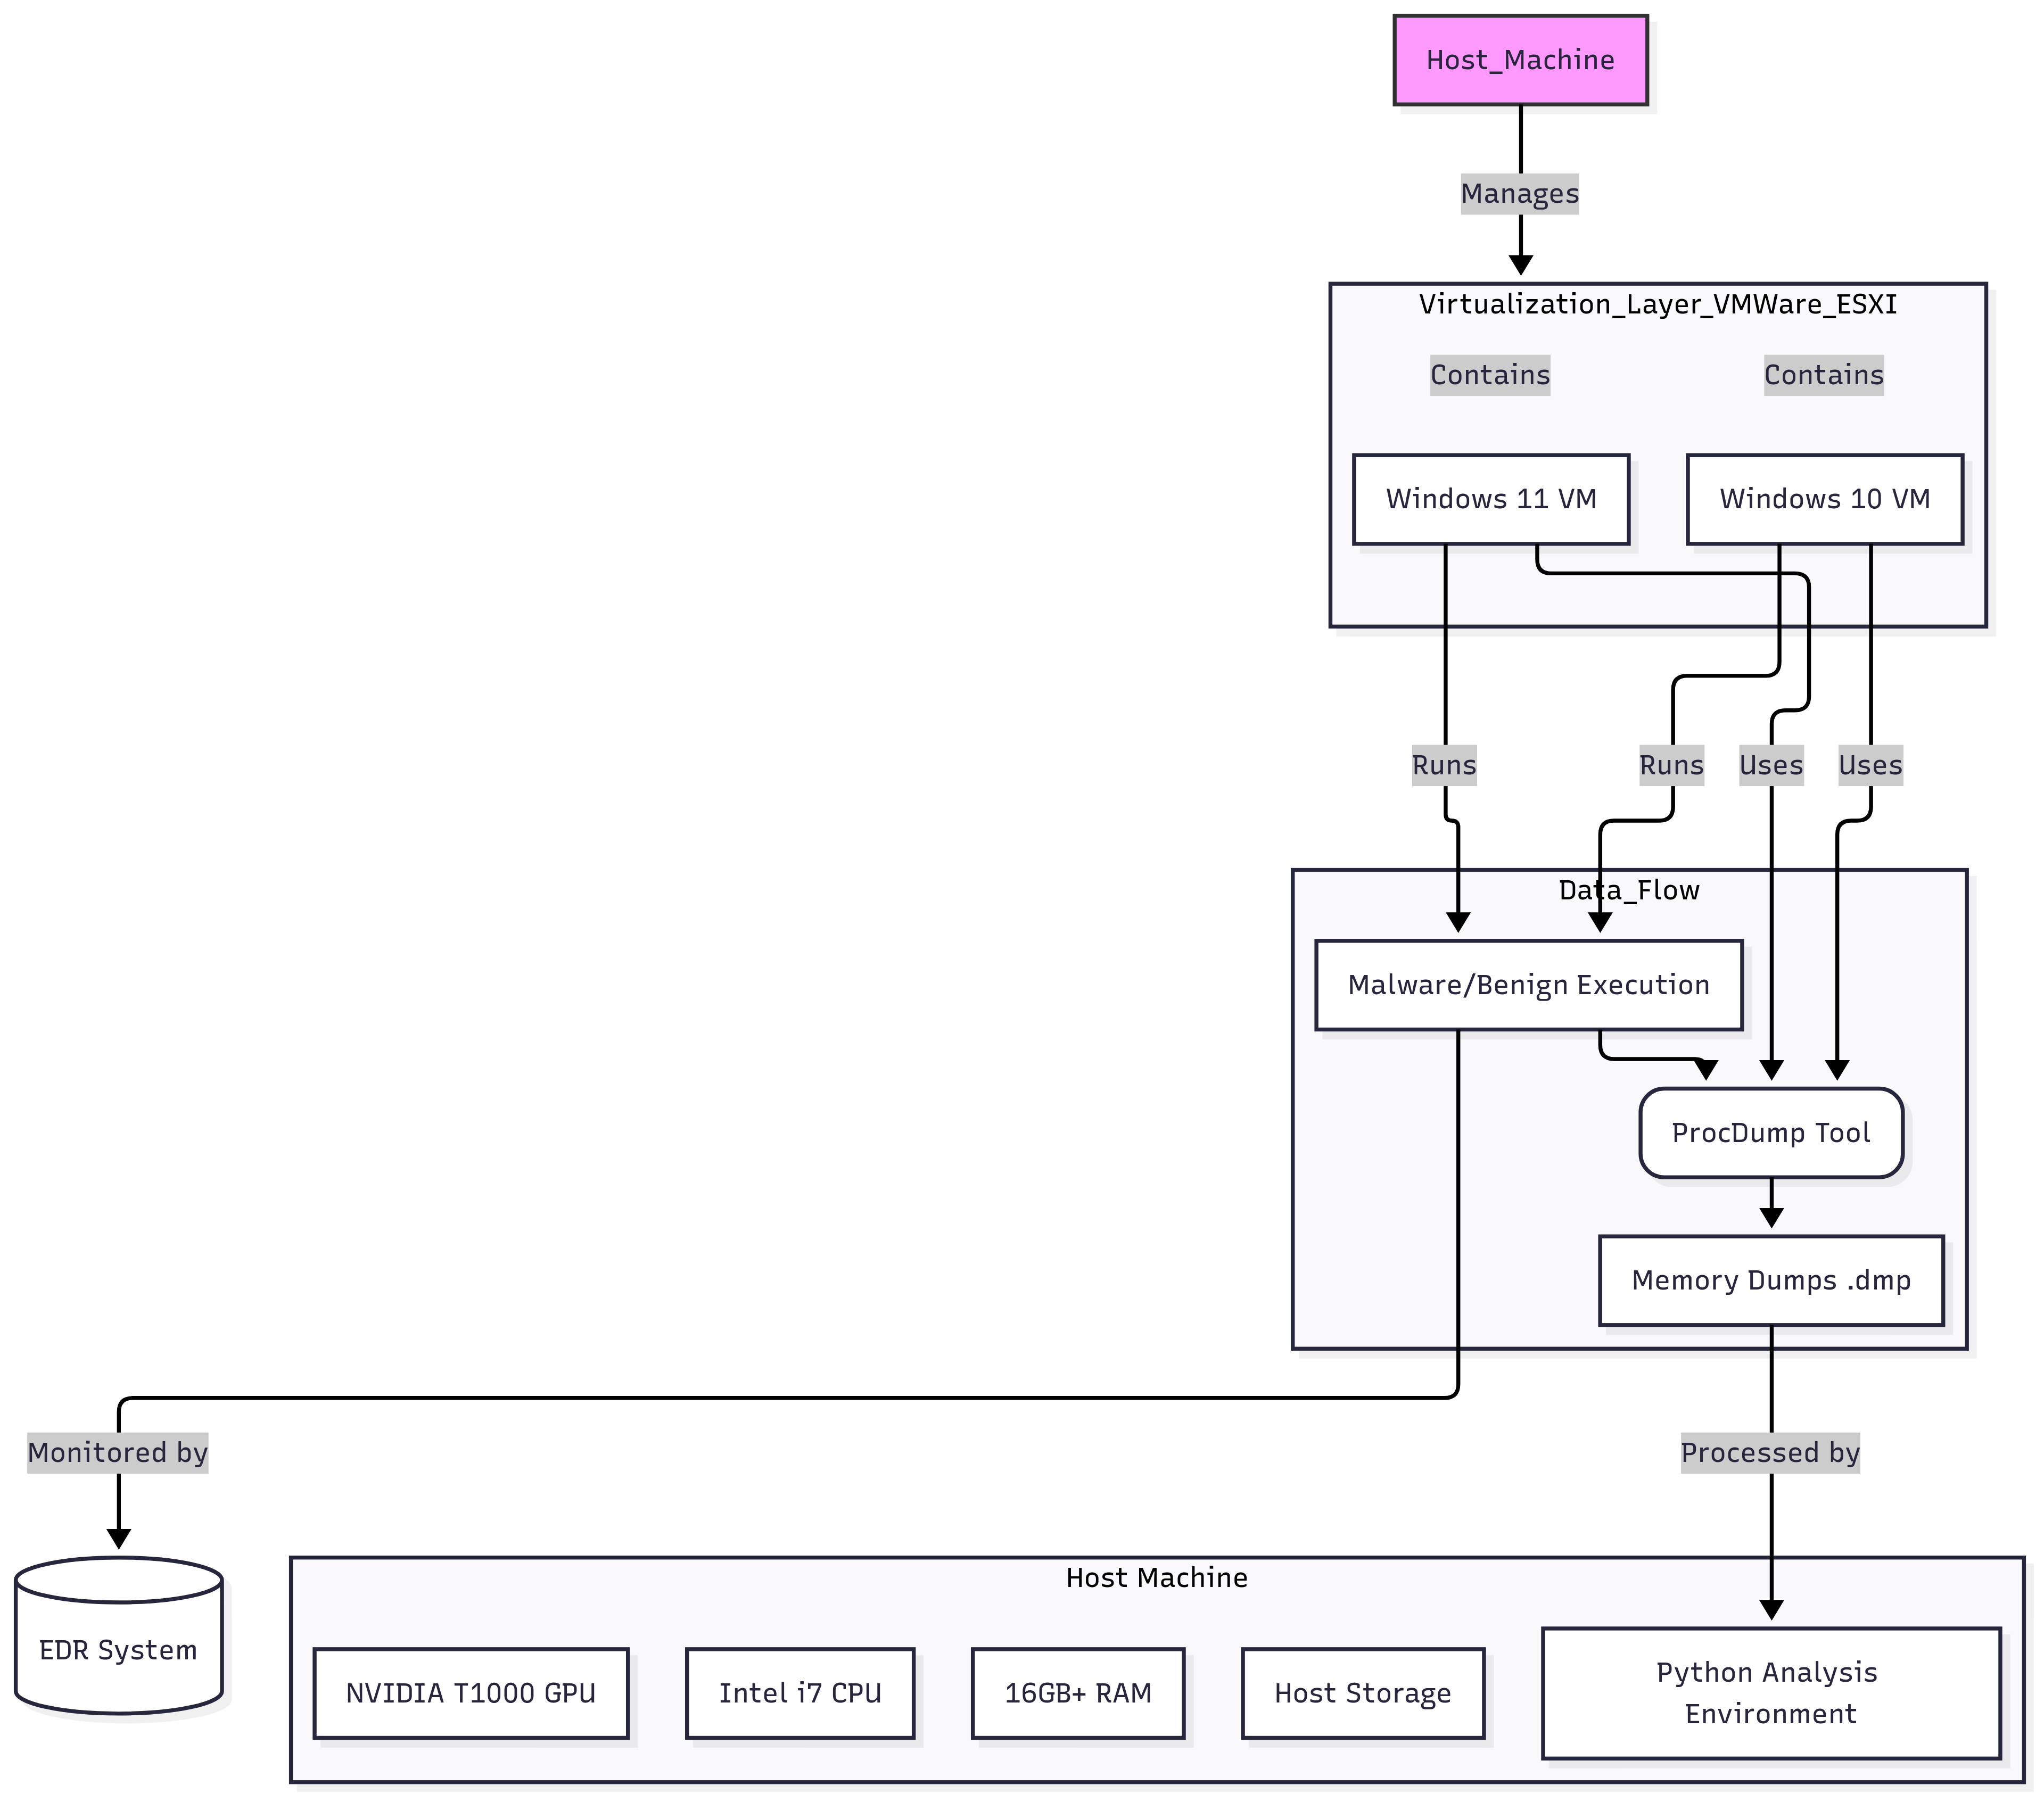
\includegraphics[width=0.8\textwidth]{../Assets/3-2.png}
  \caption{System architecture and experimental setup.}
  \label{fig:system_setup}
\end{figure}
% --- End Placeholder ---

% --- Section 3.3 ---
\section{Implementation Details}
\label{sec:implementation_details}

This section provides a detailed breakdown of the specific procedures and algorithms implemented within each phase of the proposed framework.

\subsection{Memory Dump Collection}
\label{subsec:mem_dump_collection}

The foundation of the analysis lies in obtaining high-quality memory dumps that accurately capture the runtime state of potentially malicious processes. The following systematic procedure was implemented[cite: 67]:

\begin{enumerate}
    \item \textbf{Sandbox Environment Setup:} Isolated virtual environments were crucial for safely executing malware samples. Windows 10 and Windows 11 guest operating systems were deployed using the VMWare ESXI hypervisor platform. This setup ensured that malware execution was contained and did not affect the host system or network.
    \item \textbf{Memory Allocation Strategy:} To ensure the integrity and completeness of memory dumps, particularly for larger processes or to mitigate potential effects of memory randomization techniques like ASLR, a significant amount of RAM (over 16GB) was allocated to each virtual machine during the analysis phase[cite: 67]. This large allocation aimed to provide sufficient contiguous space for process memory, potentially reducing fragmentation.
    \item \textbf{Memory Acquisition Tool Configuration:} Microsoft's ProcDump utility (version 9.0) was selected for capturing memory dumps[cite: 60]. It was executed with the `-ma` command-line argument. This specific parameter instructs ProcDump to capture a full process memory dump, which includes the entire virtual address space of the target process, encompassing both physical memory pages mapped to the process and its virtual memory contents. This comprehensive capture is vital for analyzing all aspects of the process's memory footprint.
    \item \textbf{Execution Monitoring:} Before capturing the dump, the target PE file (either malware or benign) was executed within the sandboxed VM. An Endpoint Detection and Response (EDR) system was monitored concurrently to confirm that the process had successfully launched and was actively running[cite: 60]. This step ensures that the memory dump captures the process in an active state, rather than during initialization or termination.
    \item \textbf{Dump Collection and Organization:} Once successful execution was confirmed, ProcDump was triggered to generate the memory dump file (with a `.dmp` extension). The collected dump files were systematically organized based on the corresponding malware family or benign category to maintain dataset integrity[cite: 60]. The resulting dump files varied significantly in size, typically ranging from one to several gigabytes, depending on the complexity of the executed program and the modules it loaded into memory.
\end{enumerate}

This structured process ensured that consistent and comprehensive memory snapshots were collected for each sample under analysis.

% --- Mermaid Diagram for 3.3.1 ---
% \begin{figure}[h!]
% \centering
% % \includegraphics{mem_dump_diagram.pdf} % Example include
\begin{verbatim}
graph TD
    A[Start: Setup Sandbox] --> B{Deploy Win10/11 VM (VMWare ESXI)};
    B --> C{Allocate >16GB RAM to VM};
    C --> D[Execute Target PE File in VM];
    D --> E{Monitor EDR for Execution Confirmation};
    E -- Confirmed --> F[Run ProcDump v9.0 with -ma];
    F --> G(Generate Full Process Memory Dump *.dmp);
    G --> H[Organize Dump by Family/Category];
    H --> I[End: Memory Dump Collected];

    style G fill:#ccffcc,stroke:#333,stroke-width:1px
\end{verbatim}
% \caption{Process flow for Memory Dump Collection.}
% \label{fig:mem_dump_collection}
% \end{figure}
% --- End Mermaid Diagram ---


\subsection{RGB Image Conversion}
\label{subsec:rgb_conversion}

To leverage computer vision techniques, the collected binary memory dumps were transformed into RGB image representations. This conversion allows visual patterns inherent in the binary data structure to be analyzed. The process involved the following steps[cite: 61]:

\begin{enumerate}
    \item \textbf{Binary Data Reading:} Each memory dump file (`.dmp`) was read as a sequential stream of raw bytes.
    \item \textbf{RGB Pixel Encoding:} The byte stream was processed in sequential groups of three. Each triplet of bytes was directly mapped to the Red, Green, and Blue (RGB) channels of a single pixel. The first byte determined the Red intensity (0-255), the second byte the Green intensity, and the third byte the Blue intensity. This creates a direct visual representation where pixel color corresponds to consecutive byte values.
    \item \textbf{Column Width Configuration and Optimization:} The linear sequence of pixels needs to be arranged into a 2D image format. The width (number of columns) of this image can influence the resulting visual patterns. Four different column width configurations were tested to determine an optimal representation that might best preserve structural byte patterns: 224 pixels, 300 pixels, 4096 pixels, and a "square root scheme" (where the width is approximately the square root of the total number of pixels)[cite: 61]. The 4096px width was found to be optimal in the experiments (as detailed in Chapter 4).
    \item \textbf{Image Standardization:} Regardless of the initial width and resulting height, the generated images were standardized to square dimensions (specifically $224 \times 224$ or $300 \times 300$ pixels, depending on the feature extraction input requirements) for consistent input to subsequent processing steps. Lanczos interpolation was used during resizing, as it is known for preserving image quality, especially when downscaling.
    \item \textbf{Lossless Storage:} The final standardized RGB images were saved using the Portable Network Graphics (PNG) format. PNG is a lossless compression format, ensuring that no information from the original byte-to-pixel mapping was lost during storage[cite: 61].
\end{enumerate}

This conversion process was implemented using a customized Python script, adapted from the "bin2png" concept, specifically optimized to handle the large file sizes associated with multi-gigabyte memory dumps[cite: 62]. The core logic of the conversion is captured in Algorithm \ref{alg:rgb_conversion}[cite: 63].

% --- Algorithm Placeholder ---
% Using verbatim for simplicity; consider algorithm packages like algorithm2e for better formatting
\begin{figure}[h!]
\centering
\begin{verbatim}
Algorithm 1: Memory Dump to RGB Image Conversion
-------------------------------------------------
Input: binary file 'file', target image width 'width', target square size 'targetSize'
Output: standardized square RGB image 'img_resized'

1: function ConvertToRGBImage(file, width, targetSize)
2:     data <- ReadBinary(file)
3:     numBytes <- length(data)
4:     pxCount <- floor(numBytes / 3)
5:     
6:     height <- ceil(pxCount / width)
7:     img <- CreateRGBImage(width, height)
8:     
9:     for i = 0 to pxCount - 1 do
10:        r <- data[3*i]
11:        g <- data[3*i + 1]
12:        b <- data[3*i + 2]
13:        
14:        x <- i mod width       // Column
15:        y <- floor(i / width)  // Row
16:        
17:        img[x, y] <- (r, g, b)
18:     end for
19:     
20:     img_resized <- ResizeToSquare(img, targetSize, method='Lanczos')
21:     return img_resized
22: end function
\end{verbatim}
\caption{Algorithm for converting memory dump to standardized RGB image.}
\label{alg:rgb_conversion}
\end{figure}
% --- End Algorithm Placeholder ---

% --- Mermaid Diagram for 3.3.2 ---
% \begin{figure}[h!]
% \centering
% % \includegraphics{rgb_conversion_diagram.pdf} % Example include
\begin{verbatim}
graph TD
    A[Start: Input Memory Dump (.dmp)] --> B{Read Binary Data Stream};
    B --> C{Group Bytes into Triplets (R, G, B)};
    C --> D{Map Triplets to Pixels};
    D --> E{Arrange Pixels into 2D Image (Select Width: e.g., 4096px)};
    E --> F{Resize Image to Standard Square (e.g., 224x224) using Lanczos};
    F --> G[Save as Lossless PNG Image];
    G --> H[End: Standardized RGB Image];

    style G fill:#ccffcc,stroke:#333,stroke-width:1px
\end{verbatim}
% \caption{Process flow for RGB Image Conversion.}
% \label{fig:rgb_conversion}
% \end{figure}
% --- End Mermaid Diagram ---

\subsection{Feature Extraction}
\label{subsec:feature_extraction_impl}

From the standardized RGB images, features capturing their visual characteristics were extracted. A combination of global (GIST) and local (HOG) features was used to create a comprehensive representation[cite: 24].

\begin{enumerate}
    \item \textbf{GIST Feature Extraction:} GIST features \citep{oliva2001modeling} were extracted to capture the overall spatial structure and texture of the image. A custom extractor was implemented. Multi-scale Gabor filters were applied with 8 orientations and 4 scales across each of the three RGB channels. The image was conceptually divided into a $4 \times 4$ grid, and filter responses were aggregated within each grid cell. This process resulted in a 960-dimensional feature vector (calculated as 3 channels $\times$ 16 grid cells $\times$ (8 orientations/scale * 4 scales = 32) -> Note: paper calculation seems different, 3*16*(8+8+4) is wrong, 3*16*8*4 = 1536? Or maybe feature aggregation method yields 960? Sticking to paper value for now). The extraction required approximately 1.67 seconds per image on the test system[cite: 68].
    \item \textbf{HOG Feature Extraction:} HOG features \citep{dalal2005histograms} were extracted to capture local shape information based on edge orientations. For HOG extraction, images were first resized to $256 \times 256$ pixels. The image was then divided into $32 \times 32$ pixel cells. Within each cell, gradient magnitudes and orientations were computed, and a histogram of gradients using 9 orientation bins was created. These histograms were then normalized across overlapping $2 \times 2$ blocks of cells for robustness. This procedure yielded a 1764-dimensional feature vector[cite: 69, 70]. HOG extraction took approximately 1.12 seconds per image[cite: 70].
    \item \textbf{Feature Fusion and Standardization:} The extracted 960-dimensional GIST vector and the 1764-dimensional HOG vector were concatenated to form a combined 2724-dimensional feature vector for each image. This fusion aims to leverage the complementary strengths of global and local descriptors. Finally, the combined feature vectors across the entire dataset were standardized (typically to zero mean and unit variance) to ensure all features contribute equally during machine learning model training, preventing features with larger numerical ranges from dominating the learning process[cite: 70].
\end{enumerate}

The feature extraction and fusion logic is outlined in Algorithm \ref{alg:feature_extraction}[cite: 71].

% --- Algorithm Placeholder ---
\begin{figure}[h!]
\centering
\begin{verbatim}
Algorithm 2: Feature Extraction and Fusion
-------------------------------------------
Input: standardized RGB image 'image'
Output: standardized fused feature vector 'Fc_standardized'

1: function ExtractFeatures(image)
2:     // GIST Extraction (Conceptual - details depend on implementation)
3:     gistParams <- {scales: 4, orientations: 8, grid: 4x4}
4:     Fg <- ExtractGIST(image, gistParams)  // Results in 960 dims
5:     
6:     // HOG Extraction
7:     img_resized <- Resize(image, 256x256)
8:     hogParams <- {cellSize: 32x32, blockSize: 2x2, bins: 9}
9:     Fh <- ExtractHOG(img_resized, hogParams) // Results in 1764 dims
10:    
11:    // Feature Fusion
12:    Fc <- Concatenate(Fg, Fh) // Results in 2724 dims
13:   
14:    // Standardization (applied across dataset, shown conceptually here)
15:    Fc_standardized <- Standardize(Fc) 
16:    
17:    return Fc_standardized
18: end function
\end{verbatim}
\caption{Algorithm for GIST and HOG feature extraction and fusion.}
\label{alg:feature_extraction}
\end{figure}
% --- End Algorithm Placeholder ---


% --- Mermaid Diagram for 3.3.3 ---
% \begin{figure}[h!]
% \centering
% % \includegraphics{feature_extraction_diagram.pdf} % Example include
\begin{verbatim}
graph TD
    A[Start: Input Standardized RGB Image] --> B{Feature Extraction};
    
    subgraph GIST Path
        B --> GIST_Extract(Extract GIST Features);
        GIST_Extract --> GIST_Vector[960-dim GIST Vector];
    end
    
    subgraph HOG Path
        B --> HOG_Resize(Resize Image to 256x256);
        HOG_Resize --> HOG_Extract(Extract HOG Features);
        HOG_Extract --> HOG_Vector[1764-dim HOG Vector];
    end
    
    GIST_Vector & HOG_Vector --> Fusion(Concatenate Features);
    Fusion --> Combined_Vector[2724-dim Combined Vector];
    Combined_Vector --> Standardize(Standardize Vector);
    Standardize --> F[End: Standardized Fused Feature Vector];
    
    style F fill:#ccffcc,stroke:#333,stroke-width:1px
\end{verbatim}
% \caption{Process flow for Feature Extraction and Fusion.}
% \label{fig:feature_extraction}
% \end{figure}
% --- End Mermaid Diagram ---


\subsection{Classification Algorithms}
\label{subsec:classification_algos}

The extracted and standardized 2724-dimensional feature vectors were used as input to train and evaluate several standard machine learning classification algorithms. The goal was to assess which algorithm performed best for the task of multi-class malware family classification and, subsequently, for binary classification in the context of unknown malware detection. The following five algorithms were implemented and evaluated[cite: 74]:

\begin{itemize}
    \item \textbf{Random Forest (RF):} An ensemble learning method that constructs multiple decision trees during training and outputs the class that is the mode of the classes output by individual trees. It is generally robust to overfitting and can handle high-dimensional data. An ensemble of 100 decision trees was used with default parameters provided by the implementation library (likely Scikit-learn).
    \item \textbf{Sequential Minimal Optimization (SMO):} An algorithm used for training Support Vector Machines (SVMs). It breaks down the large quadratic programming optimization problem associated with SVM training into a series of smaller sub-problems that are then solved analytically. An SMO implementation with a Radial Basis Function (RBF) kernel was used, with the regularization parameter $C$ set to 10.
    \item \textbf{Linear Support Vector Machine (Linear SVM):} A variant of SVM that uses a linear kernel function. It aims to find a hyperplane that best separates different classes in the feature space. A Linear SVM classifier was configured with the regularization parameter $C$ set to 10.
    \item \textbf{XGBoost (Extreme Gradient Boosting):} An efficient and scalable implementation of the gradient boosting framework. It builds an ensemble of decision trees sequentially, with each new tree attempting to correct the errors made by the previous ones. An XGBoost classifier with 100 estimators (trees) was used.
    \item \textbf{J48:} An open-source Java implementation of the C4.5 decision tree algorithm. It builds a single decision tree based on information entropy or gain ratio criteria. This was included primarily as a baseline single-tree classifier for comparison against the ensemble methods.
\end{itemize}

These classifiers were employed in two distinct experimental phases: firstly, for multi-class classification to identify specific known malware families (Phase 1), and secondly, for binary classification (malware vs. benign) within the UMAP-based framework for detecting unknown malware (Phase 2)[cite: 74].

% --- Mermaid Diagram for 3.3.4 ---
% \begin{figure}[h!]
% \centering
% % \includegraphics{classification_diagram.pdf} % Example include
\begin{verbatim}
graph TD
    A[Input: Standardized Feature Vectors (2724-dim)];
    A --> B{Select Classifier};
    
    subgraph Classifiers Used
        C[Random Forest (100 trees)];
        D[SMO (RBF Kernel, C=10)];
        E[Linear SVM (C=10)];
        F[XGBoost (100 estimators)];
        G[J48 (C4.5 Decision Tree)];
    end
    
    B --> C; B --> D; B --> E; B --> F; B --> G;
    
    H{Train Classifier};
    C --> H; D --> H; E --> H; F --> H; G --> H;

    I[Input: Test Feature Vectors];
    H & I --> J{Predict Class Labels};
    J --> K[Output: Classification Results (Accuracy, F1, etc.)];
    
    style K fill:#ccffcc,stroke:#333,stroke-width:1px
\end{verbatim}
% \caption{Process flow for Classification using selected algorithms.}
% \label{fig:classification_algos}
% \end{figure}
% --- End Mermaid Diagram ---

\subsection{UMAP for Unknown Malware Detection}
\label{subsec:umap_impl}

A key contribution of this research involves leveraging the UMAP technique \citep{mcinnes2018umap} to specifically enhance the detection of unknown malware samples – those belonging to families not included in the training dataset. This addresses the critical challenge of zero-day threat detection[cite: 26, 75]. The implementation involved the following steps[cite: 72]:

\begin{enumerate}
    \item \textbf{Dataset Configuration for Unknown Detection:} To simulate the scenario of encountering unknown malware, a cross-validation-like strategy was employed using folds. The dataset (containing 10 malware families + 1 benign class) was divided into three distinct folds. For each fold, 7 malware families (plus the benign class) were designated as "known" and used for training, while the remaining 3 malware families were held out as "unknown" and used exclusively for testing the model's ability to detect novel threats.
    \item \textbf{Supervised Dimensionality Reduction with UMAP:} UMAP was applied to the high-dimensional (2724-dim) feature space of the known training data. Crucially, UMAP was trained in *supervised* mode. This means that the class labels (e.g., mapping all known malware families to a single 'malware' label and benign samples to a 'benign' label for binary classification) were provided to the UMAP algorithm during the dimensionality reduction process. Supervised UMAP aims to find a low-dimensional embedding that not only preserves the structure of the data but also explicitly tries to separate the different classes provided as labels, potentially creating a more discriminative latent space for classification tasks. The target dimensionality for the UMAP embedding was set to 4 dimensions[cite: 72].
    \item \textbf{Hyperparameter Tuning:} The performance of UMAP can be sensitive to its hyperparameters. Extensive experimentation was conducted to determine the optimal configuration. The best results were achieved with `n_neighbors` set to 55, `min_dist` set to 1.0, and using the Manhattan distance metric[cite: 72, 97]. `n_neighbors` controls the balance between local and global structure preservation, while `min_dist` controls how tightly points are packed in the low-dimensional embedding.
    \item \textbf{Model Training and Evaluation:} After applying the trained UMAP transformation to both the known training data and the unseen test data (containing unknown malware families), machine learning classifiers (as described in Section \ref{subsec:classification_algos}) were trained on the resulting 4-dimensional embeddings of the known data. These classifiers were typically trained for a binary task (malware vs. benign). Finally, the trained models were evaluated on the transformed test data to assess their performance in detecting the unknown malware samples[cite: 72]. Performance metrics like accuracy, precision, recall, and F1-score were calculated specifically for this unknown detection task.
\end{enumerate}

This process, detailed in Algorithm \ref{alg:umap_detection}[cite: 73], allows for a rigorous evaluation of how UMAP-based dimensionality reduction impacts the ability of standard classifiers to generalize and identify novel threats.

% --- Algorithm Placeholder ---
\begin{figure}[h!]
\centering
\begin{verbatim}
Algorithm 3: Unknown Malware Detection with UMAP
------------------------------------------------
Input: Full Dataset (Images + Labels), Fold configuration (e.g., 7 known, 3 unseen)
Output: Performance metrics for unknown malware detection

1: function DetectUnknownMalware(fullDataset, foldConfig)
2:     all_perf <- []
3:     folds <- CreateFolds(fullDataset, foldConfig)
4:     
5:     for each fold in folds do
6:         trainData, testData_unseen <- GetTrainTestData(fold)
7:         
8:         // Prepare training data for UMAP & Classifier
9:         Xt <- ExtractFeatures(trainData.images) // Get 2724-dim features
10:        yt_binary <- ConvertToBinaryLabels(trainData.labels) // 0=benign, 1=malware
11:       
12:        // UMAP Reduction (Supervised)
13:        umap_reducer <- InitUMAP(dims=4, neighbors=55, minDist=1.0, metric='Manhattan')
14:        Xt_reduced <- umap_reducer.fit_transform(Xt, yt_binary) // Train UMAP
15:       
16:        // Train Classifier on reduced known data
17:        clf <- TrainClassifier(Xt_reduced, yt_binary) 
18:       
19:        // Prepare unseen test data
20:        Xe_unseen <- ExtractFeatures(testData_unseen.images)
21:        ye_binary_unseen <- ConvertToBinaryLabels(testData_unseen.labels)
22:       
23:        // Apply trained UMAP transformation
24:        Xe_reduced_unseen <- umap_reducer.transform(Xe_unseen) 
25:       
26:        // Test classifier on reduced unseen data
27:        pred <- clf.Predict(Xe_reduced_unseen)
28:        perf <- EvaluateMetrics(pred, ye_binary_unseen)
29:        append perf to all_perf
30:     end for
31:     
32:     return AggregatePerformance(all_perf)
33: end function
\end{verbatim}
\caption{Algorithm for applying UMAP for unknown malware detection.}
\label{alg:umap_detection}
\end{figure}
% --- End Algorithm Placeholder ---

% --- Mermaid Diagram for 3.3.5 ---
% \begin{figure}[h!]
% \centering
% % \includegraphics{umap_detection_diagram.pdf} % Example include
\begin{verbatim}
graph TD
    A[Start: Input Fused Features (2724-dim) & Labels];
    B{Split Data into Folds (Known Train / Unknown Test)};
    
    subgraph Training Phase (for each fold)
        C[Known Training Data (Features + Binary Labels)];
        D{Configure UMAP (dims=4, n=55, d=1.0, metric='Manhattan')};
        E{Train Supervised UMAP on Known Data};
        E --> F[Trained UMAP Reducer];
        C --> E; D --> E;
        F --> G{Transform Known Training Features -> 4-dim};
        G --> H[Reduced Known Training Data (4-dim)];
        H --> I{Train Binary Classifier (e.g., SVM) on Reduced Known Data};
        I --> J[Trained Classifier];
    end
    
    subgraph Testing Phase (for each fold)
        K[Unknown Test Data (Features + Binary Labels)];
        F --> L{Transform Unknown Test Features using Trained UMAP Reducer};
        K --> L;
        L --> M[Reduced Unknown Test Data (4-dim)];
        J & M --> N{Predict Labels for Reduced Unknown Data};
        N --> O[Evaluate Performance (Accuracy, F1 on Unknown Malware)];
    end
    
    B --> C & K;
    O --> P[End: Aggregated Performance Metrics];

    style J fill:#ddeeff,stroke:#333,stroke-width:1px
    style F fill:#ddeeff,stroke:#333,stroke-width:1px
    style P fill:#ccffcc,stroke:#333,stroke-width:1px
\end{verbatim}
% \caption{Process flow for UMAP-based Unknown Malware Detection.}
% \label{fig:umap_detection}
% \end{figure}
% --- End Mermaid Diagram ---
